\section{eo\-Stoch\-Tournament\-Worth\-Select$<$ EOT, Worth\-T $>$ Class Template Reference}
\label{classeo_stoch_tournament_worth_select}\index{eoStochTournamentWorthSelect@{eoStochTournamentWorthSelect}}
An instance of eo\-Select\-Perf2Worth that does selection from the Worthes using a ...  


{\tt \#include $<$eo\-Select\-From\-Worth.h$>$}

Inheritance diagram for eo\-Stoch\-Tournament\-Worth\-Select$<$ EOT, Worth\-T $>$::\begin{figure}[H]
\begin{center}
\leavevmode
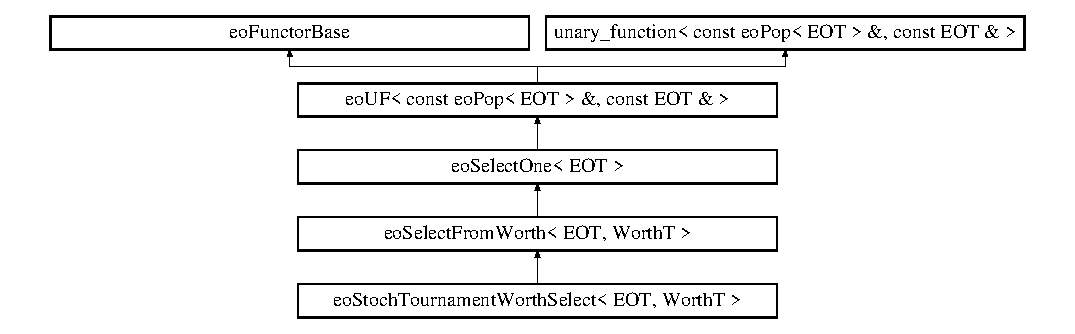
\includegraphics[height=4.04624cm]{classeo_stoch_tournament_worth_select}
\end{center}
\end{figure}
\subsection*{Public Types}
\begin{CompactItemize}
\item 
typedef std::vector$<$ Worth\-T $>$::iterator {\bf worth\-Iterator}\label{classeo_stoch_tournament_worth_select_w0}

\end{CompactItemize}
\subsection*{Public Member Functions}
\begin{CompactItemize}
\item 
{\bf eo\-Stoch\-Tournament\-Worth\-Select} ({\bf eo\-Perf2Worth}$<$ {\bf EOT}, Worth\-T $>$ \&\_\-perf2Worth, double \_\-t\-Rate)\label{classeo_stoch_tournament_worth_select_a0}

\item 
virtual const {\bf EOT} \& {\bf operator()} (const {\bf eo\-Pop}$<$ {\bf EOT} $>$ \&\_\-pop)\label{classeo_stoch_tournament_worth_select_a1}

\begin{CompactList}\small\item\em The pure virtual function that needs to be implemented by the subclass. \item\end{CompactList}\end{CompactItemize}
\subsection*{Private Attributes}
\begin{CompactItemize}
\item 
double {\bf t\-Rate}\label{classeo_stoch_tournament_worth_select_r0}

\end{CompactItemize}


\subsection{Detailed Description}
\subsubsection*{template$<$class EOT, class Worth\-T = double$>$ class eo\-Stoch\-Tournament\-Worth\-Select$<$ EOT, Worth\-T $>$}

An instance of eo\-Select\-Perf2Worth that does selection from the Worthes using a ... 

stochastic tournament, yes! 



Definition at line 128 of file eo\-Select\-From\-Worth.h.

The documentation for this class was generated from the following file:\begin{CompactItemize}
\item 
eo\-Select\-From\-Worth.h\end{CompactItemize}
